\chapter{Model Implementation and Results} \label{sec:practical}
To investigate the research question, seven \ac{ml} and \ac{dl} models were trained and validated on the three dataset sizes described in Section \ref{sec:data_sizes}.

Two types of supervised problems were considered: regression and classification. Due to the fundamental difference in the output values of models for these two tasks (one decimal number per feature in the former, several binary class predictions per feature in the latter), in order to enable comparison between the models, the terms \textit{hit} and \textit{hit rate} were introduced.

For classification models, a hit is simply a correct label prediction. A hit by a regression model was defined as a damage prediction, \(y_\text{pred}\), located within a tolerance of \(\pm0.15\) cycles from the Cycle Counter value, \(y_\text{true}\). The value of 0.15 is somewhat arbitrary and by no means an acceptable tolerance for a model in production, but in these initial stages is a sufficiently challenging but achievable goal.

The hit rate is determined by dividing the number of hits by the total number of predictions.

A results table for regression problems includes one \(R^2\) value (Section \ref{sec:polyreg}) to measure the quality of the fit and one mean hit rate (MHR), the mean of the feature-wise hit rates. With error defined as the difference between \(Y_\text{pred}\) and \(Y_\text{true}\), the table also contains a rows for mean absolute error (MAE) per feature and the hit rate (HR) per feature.

Results tables for the classification problem contain rows for the hit rate per feature and the mean absolute error per feature, as well as one value for the total hit rate. Since the class labels generated are ordinal (see Section \ref{sec:data:classification_rep}), error for classification models is also defined as the difference between \(Y_\text{pred}\) and \(Y_\text{true}\): a prediction \(y_\text{pred} = 3\) with a true class of \(y_\text{true} = 1\) would carry an absolute error of 2.

The programming language Python (version 3.7.5) was used for developing the models. For polynomial regression and \ac{mlp} models, the \texttt{scikit-learn} package (version 0.22.1) was used. The \ac{cnn}s were developed using \texttt{tensorflow} (version 1.15.0).

\ac{cnn}-based models were trained using a GeForce GTX 950M GPU, which completed the training substantially faster (approximately four hours) than an Intel i9-9900T CPU. For the \ac{mlp} and polynomial regression models, training was generally completed in under one minute on the CPU. (There may be room for GPU optimisation of the polynomial regression or \ac{mlp} models for better comparability and training a full-scale production model, but this was deemed unnecessary for the current research stage.)

Where results are documented in tables or plots, those stemming from the training dataset are ignored; only validation results are shown.

In the scatter plots, a perfect model would be shown by all data points lying on the line \(x = y\). The closer the points are to this line, the better the model's fit.

\section{Polynomial Regression} \label{sec:model:polyreg}
The first model implemented was a supervised machine learning method implemented with the \texttt{PolynomialFeatures} and \texttt{LinearRegression} classes from \texttt{scikit-learn}, based on the polynomial regression method as described in Section \ref{sec:polyreg}.

\subsection{Regression: Key Values} \label{sec:model:polyreg:kvs}
The input was a dataframe of key values gathered from the \ac{ehm} data. The values were selected based on their use in the Cycle Counter (maxima and exchange rates) or based on further analyses of flight data comparing phase lengths to damage.

For each flight, the input values were:

\begin{itemize}
    \item the maximum values of ALT, NH, P30 and T30;
    \item the exchange rates of NH, P30 and T30;
    \item the lengths of the taxi out, climb and cruise phases.
\end{itemize}

Its output values were seven decimal values representing damage predictions for all seven features.

Results are shown in Tables \ref{tab:polyreg:kvs_comp}, \ref{tab:polyreg:kvs_red} and \ref{tab:polyreg:kvs_vred}; predictions \(Y_{\text{pred}}\) are plotted against Cycle Counter values \(Y_{\text{true}}\) in Figure \ref{fig:polyreg_keyval_reg_scatter_complete}. The model was tested for polynomial degrees from 1 to 5; \(R^2\) increased with each degree for the training data, but peaked at degree 3 for all three dataset sizes before overfitting. Only the results corresponding to these degrees are shown.

\begin{table}
    \begin{center}
        \caption{\label{tab:polyreg:kvs_comp} Results from the polynomial regression on key values with the complete dataset (degree 3, \(R^2 = 0.252\), \(\text{MHR} = 0.810\)).}
        \begin{tabular}{ >{\bfseries}c c c c c c c c }
            \multirow{2}{*}{\textbf{Measure}} & \multicolumn{7}{c}{\textbf{Feature number}} \\
             & 1 & 2 & 3 & 4 & 5 & 6 & 7 \\
            \midrule
            MAE & 0.112 & 0.137 & 0.068 & 0.059 & 0.052 & 0.229 & 0.222 \\
            % MSE & 0.038 & 0.06 & 0.013 & 0.007 & 0.006 & 0.166 & 0.155 \\
            HR  & 0.859 & 0.798 & 0.967 & 0.977 & 0.986 & 0.525 & 0.556 \\
            \\
        \end{tabular}

        \caption{\label{tab:polyreg:kvs_red} Results from the polynomial regression on key values with the reduced dataset (degree 3, \(R^2 = 0.064\), \(\text{MHR} = 0.789\)).}
        \begin{tabular}{ >{\bfseries}c c c c c c c c }
            \multirow{2}{*}{\textbf{Measure}} & \multicolumn{7}{c}{\textbf{Feature number}} \\
             & 1 & 2 & 3 & 4 & 5 & 6 & 7 \\
            \midrule
            MAE & 0.127 & 0.16 & 0.073 & 0.071 & 0.06 & 0.255 & 0.256 \\
            % MSE & 0.071 & 0.136 & 0.012 & 0.022 & 0.011 & 0.224 & 0.208 \\
            HR  & 0.822 & 0.765 & 0.95 & 0.963 & 0.969 & 0.52 & 0.534 \\
            \\
        \end{tabular}

        \caption{\label{tab:polyreg:kvs_vred} Results from the polynomial regression on key values with the greatly reduced dataset (degree 3, \(R^2 = -0.198\), \(\text{MHR} = 0.748\)).}
        \begin{tabular}{ >{\bfseries}c c c c c c c c }
            \multirow{2}{*}{\textbf{Measure}} & \multicolumn{7}{c}{\textbf{Feature number}} \\
             & 1 & 2 & 3 & 4 & 5 & 6 & 7 \\
            \midrule
            MAE & 0.196 & 0.231 & 0.123 & 0.098 & 0.093 & 0.365 & 0.393 \\
            % MSE & 0.583 & 0.723 & 0.234 & 0.086 & 0.074 & 1.032 & 1.899 \\
            HR  & 0.801 & 0.722 & 0.924 & 0.93 & 0.944 & 0.444 & 0.47 \\
            \\
        \end{tabular}
    \end{center}
\end{table}

\begin{figure}
    \centering
    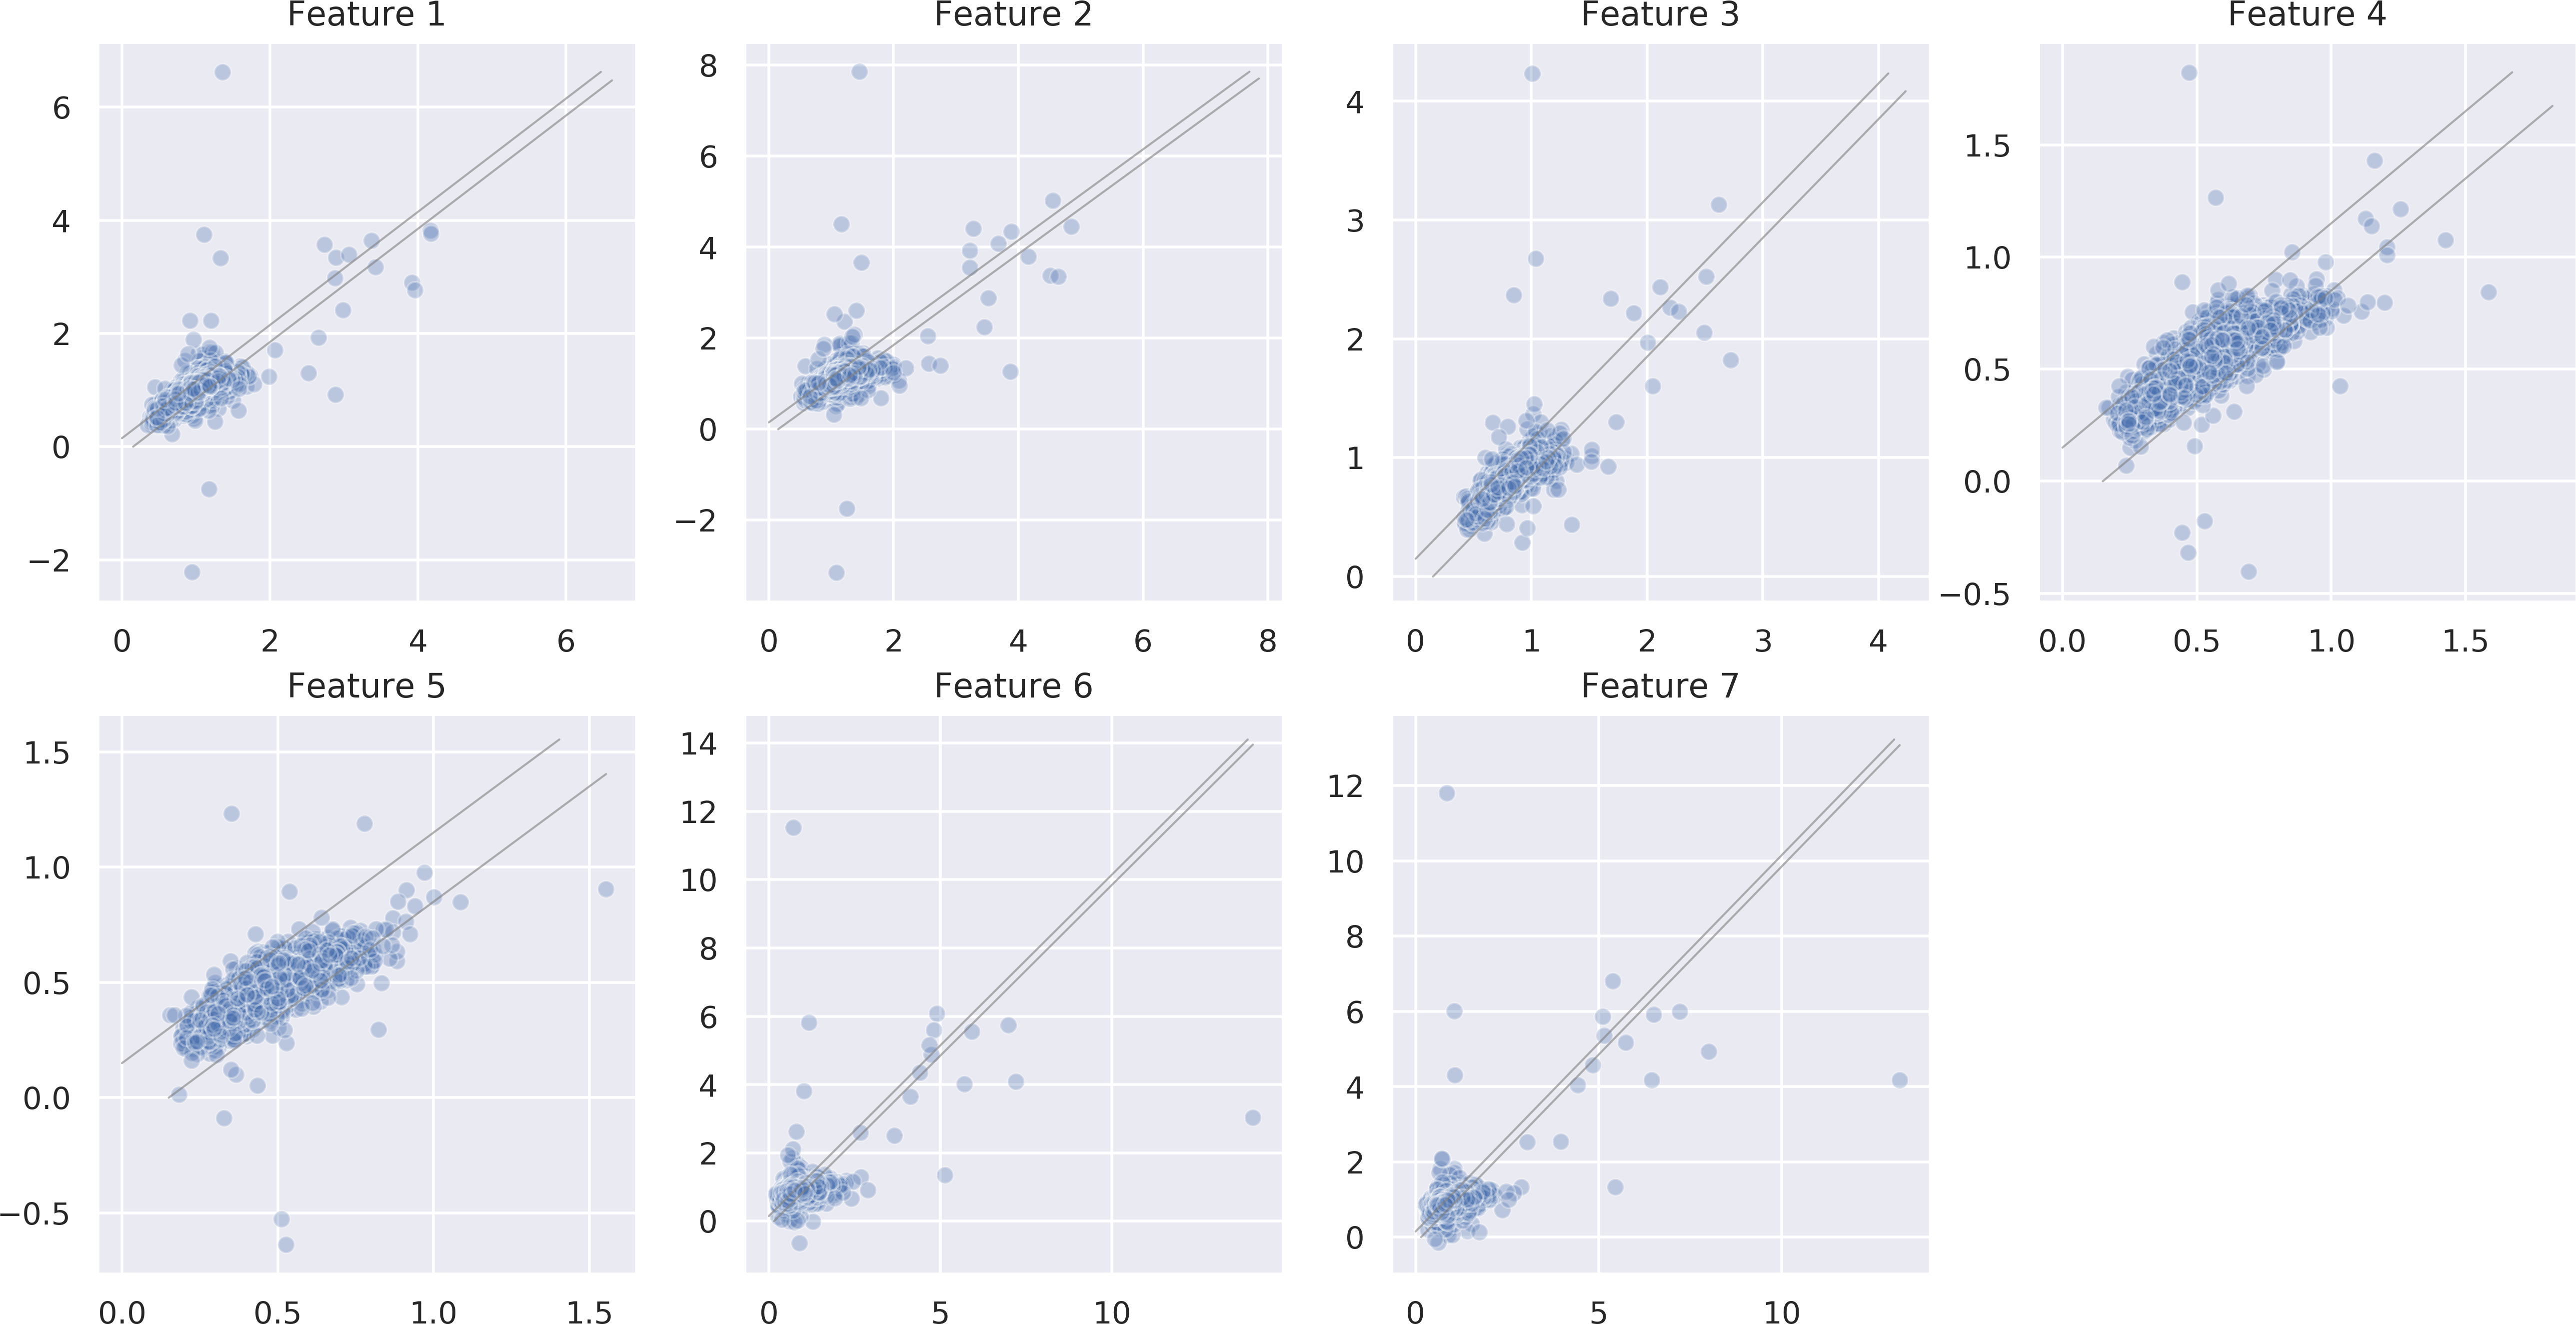
\includegraphics[width=\textwidth]{polyreg_keyval_reg_scatter_complete}
    \caption{\label{fig:polyreg_keyval_reg_scatter_complete} Scatter plots of \(Y_\text{true}\) (\(x\)-axis) versus \(Y_\text{pred}\) (\(y\)-axis) from the complete key value dataset for all seven features, as predicted by the polynomial regression model. Diagonal lines represent the \(\pm0.15\) tolerance for a hit.}
\end{figure}

\subsection{Regression: Key Values and Features} \label{sec:model:polyreg:kvfs}
For this model, the same input values as in Section \ref{sec:model:polyreg:kvs} were used, with the addition of Cycle Counter values from features 1, 4 and 6. Output values were four damage predictions for the remaining features (numbers 2, 3, 5 and 7).

Results are shown in Tables \ref{tab:polyreg:kvfs_comp}, \ref{tab:polyreg:kvfs_red} and \ref{tab:polyreg:kvfs_vred}; predictions \(Y_{\text{pred}}\) are plotted against Cycle Counter values \(Y_{\text{true}}\) in Figure \ref{fig:polyreg_keyvalfeat_reg_scatter_complete}. This model was also tested for polynomial degrees from 1 to 5; again, \(R^2\) increased with each degree for the training data, but peaked at degree 2 for the complete dataset and degree 1 for the reduced and greatly reduced datasets before overfitting.

\begin{table}
    \begin{center}
        \caption{\label{tab:polyreg:kvfs_comp} Results from the polynomial regression on key values including features 1, 4 and 6 with the complete dataset (degree 2, \(R^2 = 0.893\), \(\text{MHR} = 0.977\)).}
        \begin{tabular}{ >{\bfseries}c c c c c }
            \multirow{2}{*}{\textbf{Measure}} & \multicolumn{4}{c}{\textbf{Feature number}} \\
             & 2 & 3 & 5 & 7 \\
            \midrule
            MAE & 0.037 & 0.047 & 0.033 & 0.086 \\
            % MSE & 0.002 & 0.004 & 0.002 & 0.013 \\
            HR  & 0.997 & 0.991 & 0.999 & 0.919 \\
            \\
        \end{tabular}

        \caption{\label{tab:polyreg:kvfs_red} Results from the polynomial regression on key values including features 1, 4 and 6 with the reduced dataset (degree 1, \(R^2 = 0.864\), \(\text{MHR} = 0.968\)).}
        \begin{tabular}{ >{\bfseries}c c c c c }
            \multirow{2}{*}{\textbf{Measure}} & \multicolumn{4}{c}{\textbf{Feature number}} \\
             & 2 & 3 & 5 & 7 \\
            \midrule
            MAE & 0.047 & 0.05 & 0.036 & 0.094 \\
            % MSE & 0.005 & 0.005 & 0.002 & 0.018 \\
            HR  & 0.99 & 0.991 & 1.0 & 0.89 \\
            \\
        \end{tabular}

        \caption{\label{tab:polyreg:kvfs_vred} Results from the polynomial regression on key values including features 1, 4 and 6 with the greatly reduced dataset (degree 1, \(R^2 = 0.850\), \(\text{MHR} = 0.974\)).}
        \begin{tabular}{ >{\bfseries}c c c c c }
            \multirow{2}{*}{\textbf{Measure}} & \multicolumn{4}{c}{\textbf{Feature number}} \\
             & 2 & 3 & 5 & 7 \\
            \midrule
            MAE & 0.041 & 0.048 & 0.036 & 0.087 \\
            % MSE & 0.004 & 0.005 & 0.002 & 0.02 \\
            HR  & 0.99 & 0.99 & 1.0 & 0.917 \\
            \\
        \end{tabular}
    \end{center}
\end{table}

\begin{figure}
    \centering
    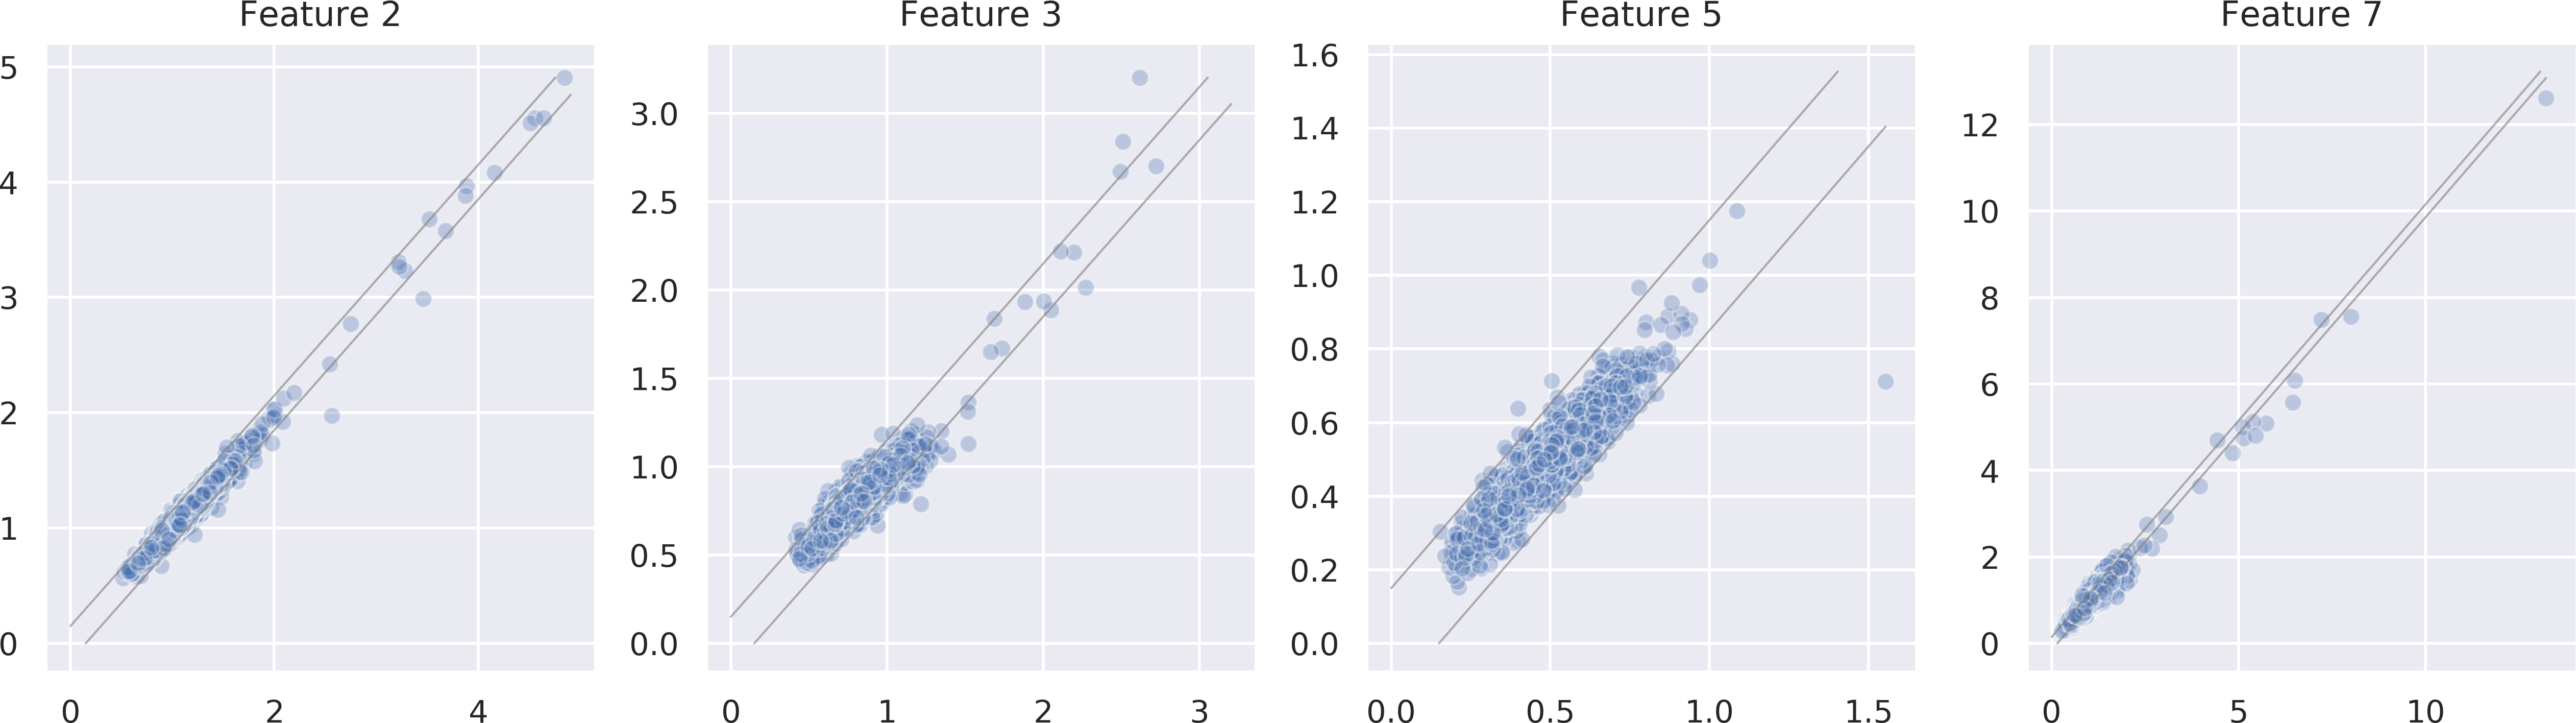
\includegraphics[width=\textwidth]{polyreg_keyvalfeat_reg_scatter_complete}
    \caption{\label{fig:polyreg_keyvalfeat_reg_scatter_complete} Scatter plots of \(Y_\text{true}\) (\(x\)-axis) versus \(Y_\text{pred}\) (\(y\)-axis) from the complete dataset comprising key values and features 1, 4 and 6, showing the polynomial regression model's damage prediction for features 2, 3, 5 and 7. Diagonal lines represent the \(\pm0.15\) tolerance for a hit.}
\end{figure}

\section{Multilayer Perceptron}
Using the \texttt{MLPRegressor} class from \texttt{scikit-learn}, three \ac{mlp}s were constructed. These contained two hidden layers of 100 nodes each and were trained until either convergence occurred, defined in this case as no improvement in loss by more than \num{1e-6} for ten epochs, or until the 500th epoch was reached.

\subsection{Regression: Key Values} \label{sec:model:mlp_kvs}
The same dataframe as defined in \ref{sec:model:polyreg:kvs} was used as an input, with an output of seven damage values.

Results for the validation dataset are shown in Tables \ref{tab:mlpreg:kvs_comp}, \ref{tab:mlpreg:kvs_red} and \ref{tab:mlpreg:kvs_vred}; predictions \(Y_{\text{pred}}\) are plotted against Cycle Counter values \(Y_{\text{true}}\) in Figure \ref{fig:mlp_keyval_reg_scatter}.

\begin{table}
    \begin{center}
        \caption{\label{tab:mlpreg:kvs_comp} Results from the \ac{mlp} regression on key values with the complete dataset (235 epochs, \(R^2 = 0.474\), \(\text{MHR} = 0.801\)).}
        \begin{tabular}{ >{\bfseries}c c c c c c c c }
            \multirow{2}{*}{\textbf{Measure}} & \multicolumn{7}{c}{\textbf{Feature number}} \\
            & 1 & 2 & 3 & 4 & 5 & 6 & 7 \\
            \midrule
            MAE & 0.115 & 0.135 & 0.069 & 0.058 & 0.051 & 0.233 & 0.227 \\
            % MSE & 0.028 & 0.044 & 0.01 & 0.006 & 0.005 & 0.111 & 0.107 \\
            HR  & 0.83 & 0.782 & 0.963 & 0.978 & 0.99 & 0.524 & 0.537 \\
            \\
        \end{tabular}

        \caption{\label{tab:mlpreg:kvs_red} Results from the \ac{mlp} regression on key values with the reduced dataset (276 epochs, \(R^2 = 0.128\), \(\text{MHR} = 0.781\)).}
        \begin{tabular}{ >{\bfseries}c c c c c c c c }
            \multirow{2}{*}{\textbf{Measure}} & \multicolumn{7}{c}{\textbf{Feature number}} \\
            & 1 & 2 & 3 & 4 & 5 & 6 & 7 \\
            \midrule
            MAE & 0.123 & 0.151 & 0.074 & 0.065 & 0.056 & 0.247 & 0.246 \\
            % MSE & 0.044 & 0.079 & 0.01 & 0.007 & 0.006 & 0.11 & 0.111 \\
            HR  & 0.825 & 0.751 & 0.945 & 0.968 & 0.983 & 0.497 & 0.496 \\
            \\
        \end{tabular}

        \caption{\label{tab:mlpreg:kvs_vred} Results from the \ac{mlp} regression on key values with the greatly reduced dataset (399 epochs, \(R^2 = -0.272\), \(\text{MHR} = 0.771\)).}
        \begin{tabular}{ >{\bfseries}c c c c c c c c }
            \multirow{2}{*}{\textbf{Measure}} & \multicolumn{7}{c}{\textbf{Feature number}} \\
            & 1 & 2 & 3 & 4 & 5 & 6 & 7 \\
            \midrule
            MAE & 0.129 & 0.153 & 0.085 & 0.069 & 0.06 & 0.274 & 0.267 \\
            % MSE & 0.04 & 0.063 & 0.016 & 0.01 & 0.006 & 0.168 & 0.21 \\
            HR  & 0.805 & 0.755 & 0.934 & 0.954 & 0.98 & 0.464 & 0.507 \\
            \\
        \end{tabular}
    \end{center}
\end{table}

\begin{figure}
    \centering
    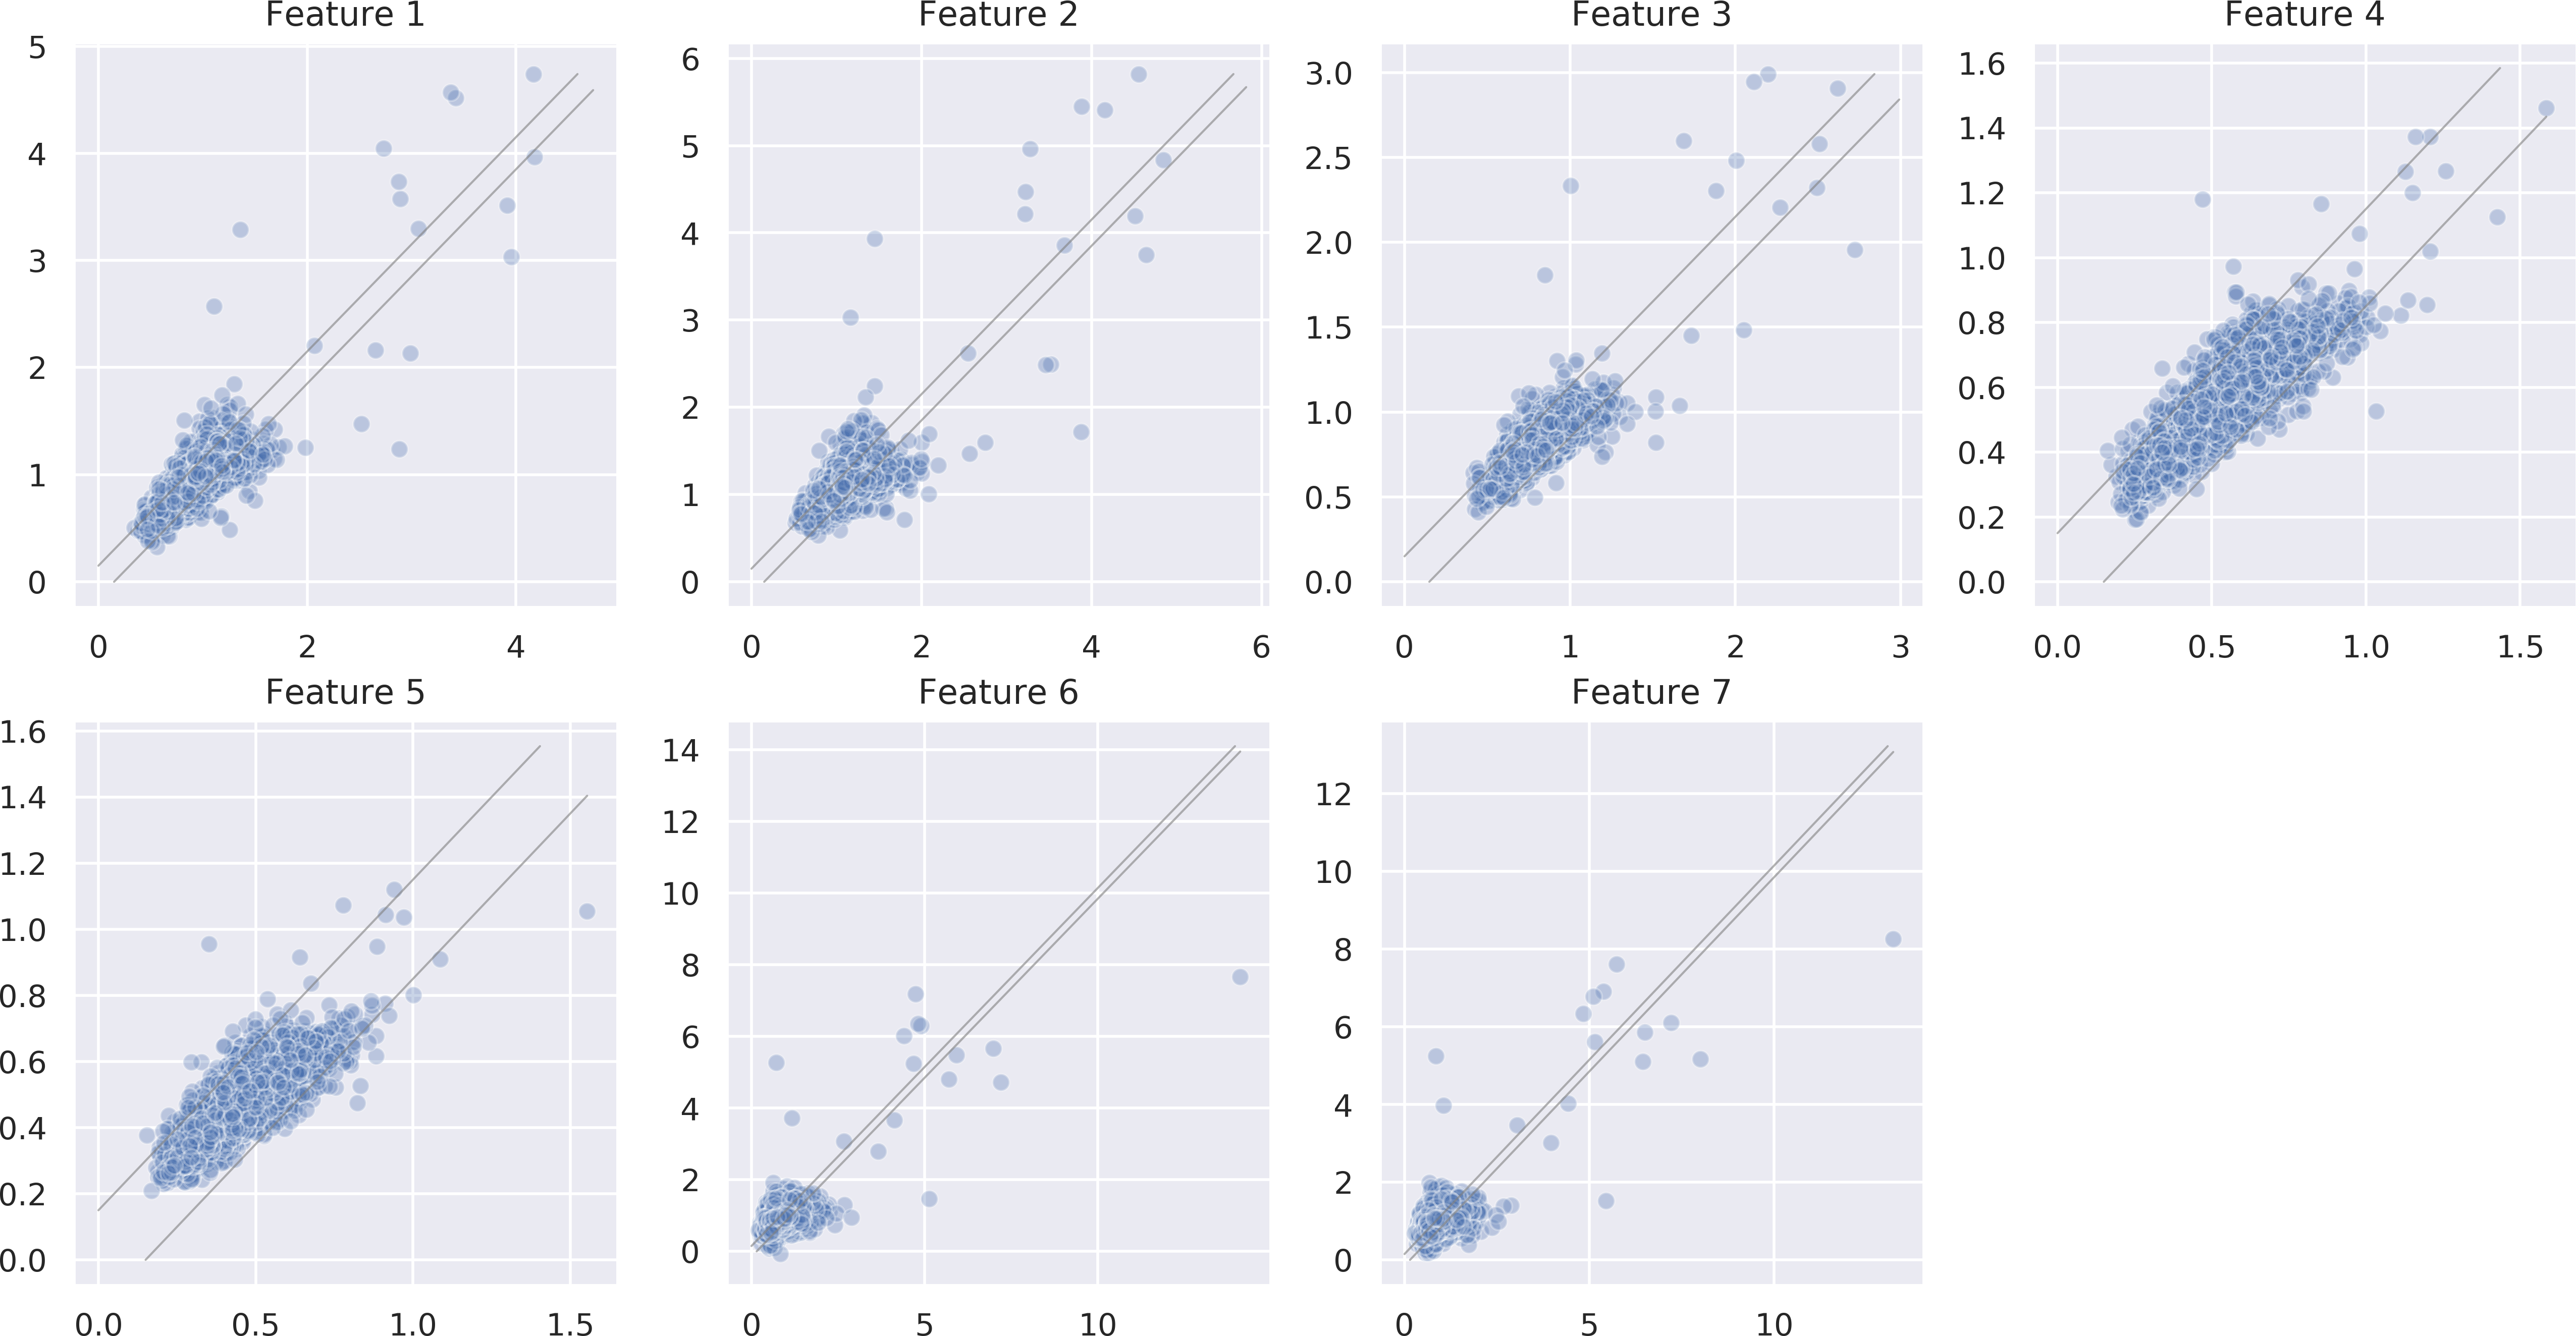
\includegraphics[width=\textwidth]{mlp_keyval_reg_scatter}
    \caption{\label{fig:mlp_keyval_reg_scatter} Scatter plots of \(Y_\text{true}\) (\(x\)-axis) versus \(Y_\text{pred}\) (\(y\)-axis) from the complete key value dataset for all seven features, as predicted by the \ac{mlp}. Diagonal lines represent the \(\pm0.15\) tolerance for a hit.}
\end{figure}

\subsection{Regression: Key Values and Features} \label{sec:model:mlp_kvfs}
The same dataframe as defined in \ref{sec:model:polyreg:kvfs} was used as an input, with an output of four damage values (features 2, 3, 5 and 7).

Results for the validation dataset are shown in Tables \ref{tab:mlpreg:kvfs_comp}, \ref{tab:mlpreg:kvfs_red} and \ref{tab:mlpreg:kvfs_vred}; predictions \(Y_{\text{pred}}\) are plotted against Cycle Counter values \(Y_{\text{true}}\) in Figure \ref{fig:mlp_keyvalfeat_reg_scatter}.

\begin{table}
    \begin{center}
        \caption{\label{tab:mlpreg:kvfs_comp} Results from the \ac{mlp} regression on key values including features 1, 4 and 6 with the complete dataset (198 epochs, \(R^2 = 0.890\), \(\text{MHR} = 0.970\)).}
        \begin{tabular}{ >{\bfseries}c c c c c }
            \multirow{2}{*}{\textbf{Measure}} & \multicolumn{4}{c}{\textbf{Feature number}} \\
             & 2 & 3 & 5 & 7 \\
            \midrule
            MAE & 0.037 & 0.049 & 0.033 & 0.095 \\
            % MSE & 0.003 & 0.004 & 0.002 & 0.017 \\
            HR  & 0.997 & 0.991 & 0.999 & 0.893 \\
            \\
        \end{tabular}

        \caption{\label{tab:mlpreg:kvfs_red} Results from the \ac{mlp} regression on key values including features 1, 4 and 6 with the reduced dataset (229 epochs, \(R^2 = 0.865\), \(\text{MHR} = 0.962\)).}
        \begin{tabular}{ >{\bfseries}c c c c c }
            \multirow{2}{*}{\textbf{Measure}} & \multicolumn{4}{c}{\textbf{Feature number}} \\
             & 2 & 3 & 5 & 7 \\
            \midrule
            MAE & 0.044 & 0.053 & 0.037 & 0.1 \\
            % MSE & 0.004 & 0.005 & 0.002 & 0.02 \\
            HR  & 0.99 & 0.988 & 0.997 & 0.873 \\
            \\
        \end{tabular}

        \caption{\label{tab:mlpreg:kvfs_vred} Results from the \ac{mlp} regression on key values including features 1, 4 and 6 with the greatly reduced dataset (500 epochs, \(R^2 = 0.740\), \(\text{MHR} = 0.949\)).}
        \begin{tabular}{ >{\bfseries}c c c c c }
            \multirow{2}{*}{\textbf{Measure}} & \multicolumn{4}{c}{\textbf{Feature number}} \\
             & 2 & 3 & 5 & 7 \\
            \midrule
            MAE & 0.052 & 0.06 & 0.044 & 0.117 \\
            % MSE & 0.005 & 0.007 & 0.003 & 0.052 \\
            HR  & 0.987 & 0.97 & 0.997 & 0.844 \\
            \\
        \end{tabular}
    \end{center}
\end{table}

\begin{figure}
    \centering
    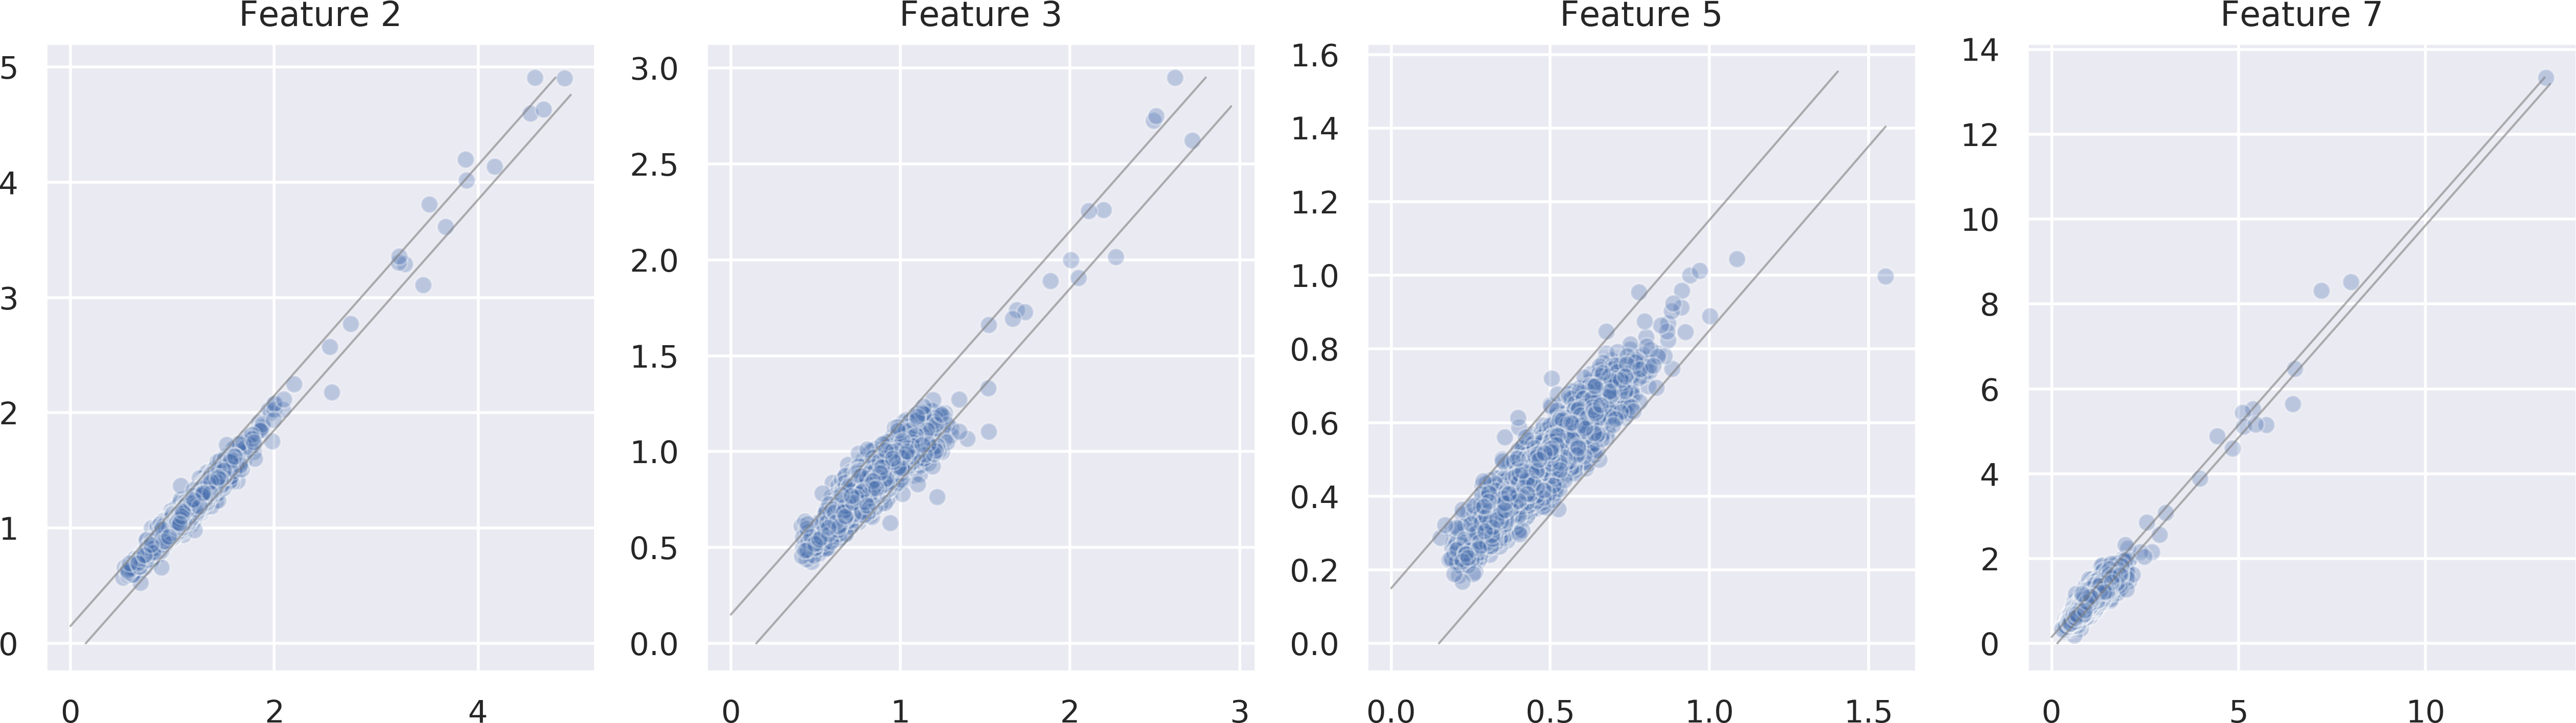
\includegraphics[width=\textwidth]{mlp_keyvalfeat_reg_scatter}
    \caption{\label{fig:mlp_keyvalfeat_reg_scatter} Scatter plots of \(Y_\text{true}\) (\(x\)-axis) versus \(Y_\text{pred}\) (\(y\)-axis) from the complete dataset comprising key values and features 1, 4 and 6, showing features 2, 3, 5 and 7 predicted by the \ac{mlp}. Diagonal lines represent the \(\pm0.15\) tolerance for a hit.}
\end{figure}

\subsection{Regression: Concatenated Multivariate Time Series} \label{sec:model:mlpreg:mts}
As input to this \ac{mlp}, the downsampled time series of all four parameters were included simultaneously by normalising (with respect to the entire dataset) and concatenating them, resulting in a one-dimensional input of 324 downsampled values. Since the model is not based on a \ac{cnn}, dynamic characteristics such as the downwards-pointing spikes in T30 (from Figure \ref{fig:high_low_dmg_T30}) cannot be learned.

The output consisted of seven decimal damage values.

\begin{figure}
    \centering
    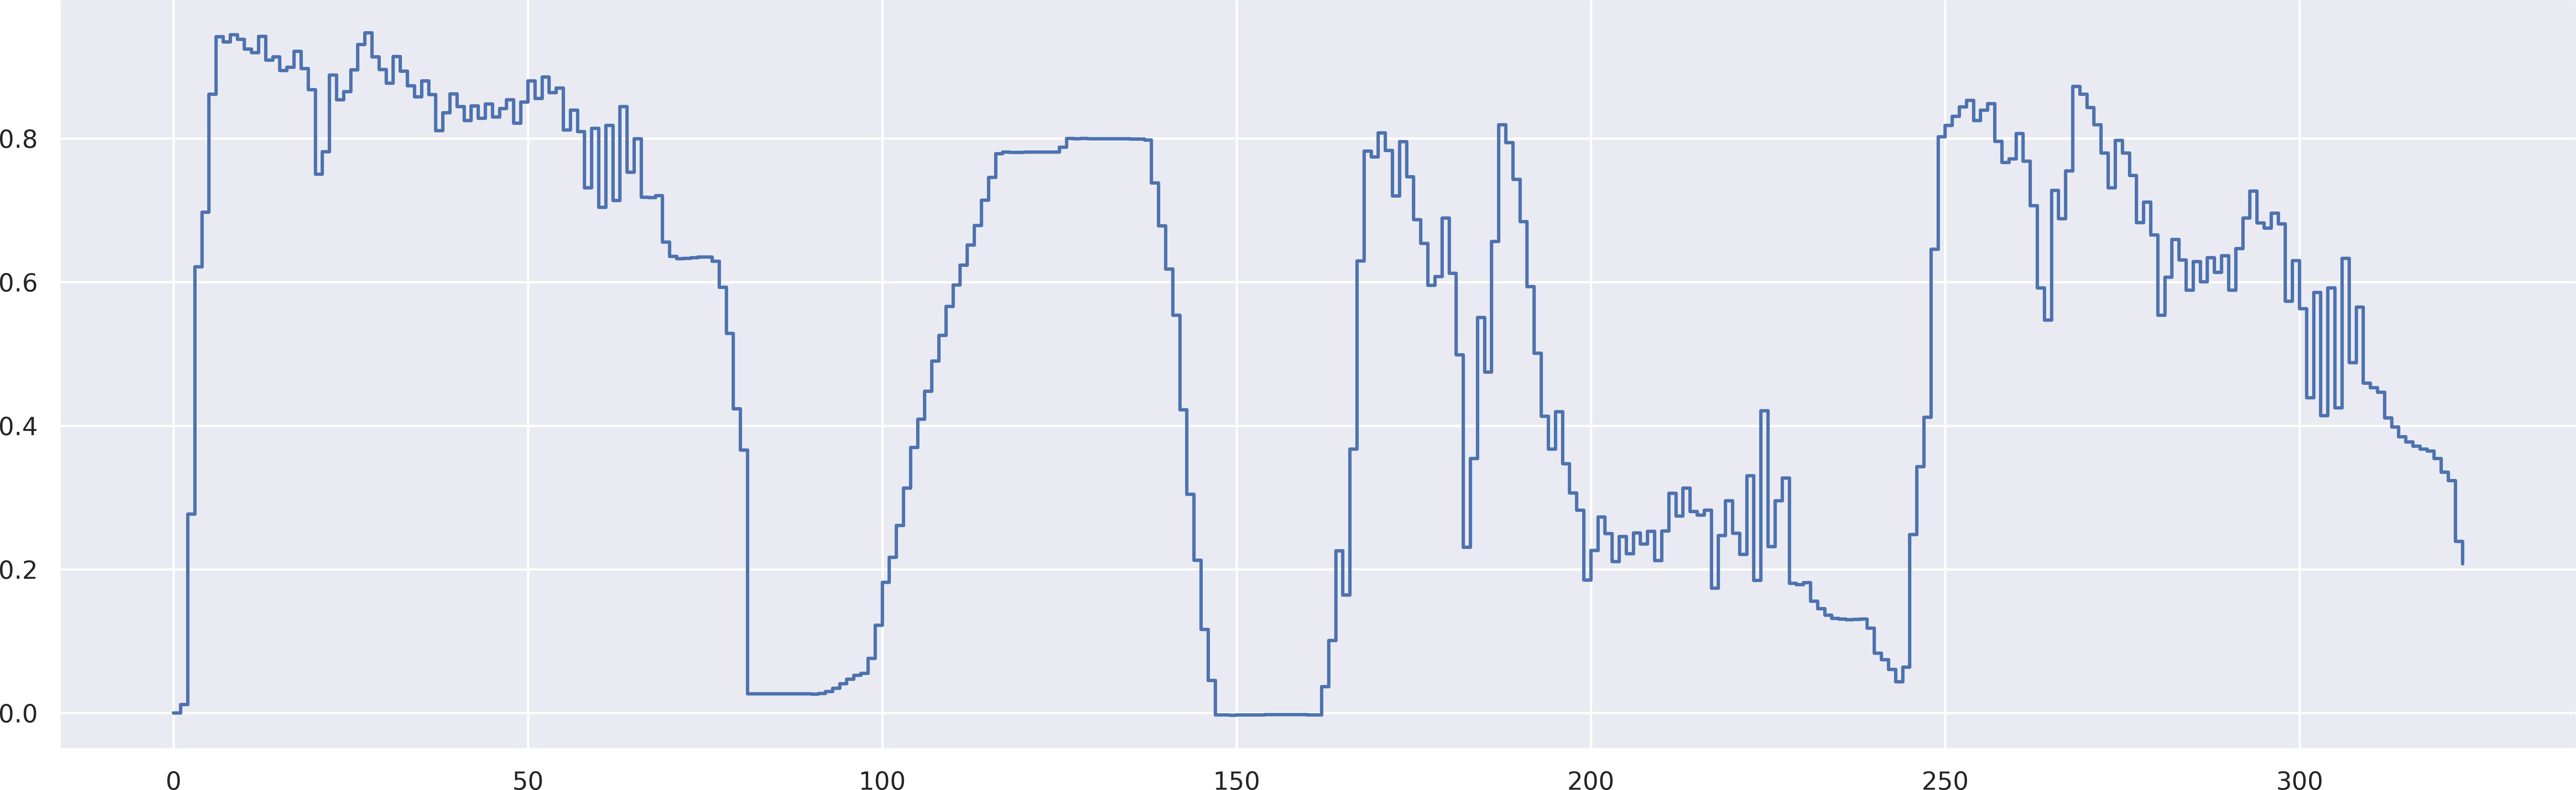
\includegraphics[width=\textwidth]{concat_mts_0815}
    \caption{\label{fig:concat_mts_0815} Concatenated, normalised, downsampled parameters NH, ALT, P30 and T30 from Flight 0815 for input to the mutlilayer perceptron.}
\end{figure}

Results are shown in Tables \ref{tab:mlpreg:mts_comp}, \ref{tab:mlpreg:mts_red} and \ref{tab:mlpreg:mts_vred}; predictions \(Y_{\text{pred}}\) are plotted against Cycle Counter values \(Y_{\text{true}}\) in Figure \ref{fig:mlp_mts_reg_scatter}.

\begin{table}
    \begin{center}
        \caption{\label{tab:mlpreg:mts_comp} Results from the \ac{mlp} regression on the concatenated multivariate time series with the complete dataset (\(R^2 = 0.301\), \(\text{MHR} = 0.799\)).}
        \begin{tabular}{ >{\bfseries}c c c c c c c c }
            \multirow{2}{*}{\textbf{Measure}} & \multicolumn{7}{c}{\textbf{Feature number}} \\
            & 1 & 2 & 3 & 4 & 5 & 6 & 7 \\
            \midrule
            MAE & 0.094 & 0.119 & 0.067 & 0.099 & 0.078 & 0.227 & 0.223 \\
            % MSE & 0.018 & 0.029 & 0.008 & 0.016 & 0.01 & 0.133 & 0.122 \\
            HR  & 0.893 & 0.82 & 0.969 & 0.882 & 0.944 & 0.542 & 0.545 \\
            \\
        \end{tabular}

        \caption{\label{tab:mlpreg:mts_red} Results from the \ac{mlp} regression on the concatenated multivariate time series with the reduced dataset (\(R^2 = 0.357\), \(\text{MHR} = 0.790\)).}
        \begin{tabular}{ >{\bfseries}c c c c c c c c }
            \multirow{2}{*}{\textbf{Measure}} & \multicolumn{7}{c}{\textbf{Feature number}} \\
            & 1 & 2 & 3 & 4 & 5 & 6 & 7 \\
            \midrule
            MAE & 0.098 & 0.121 & 0.067 & 0.099 & 0.078 & 0.231 & 0.232 \\
            % MSE & 0.019 & 0.03 & 0.008 & 0.016 & 0.01 & 0.127 & 0.121 \\
            HR  & 0.882 & 0.803 & 0.969 & 0.876 & 0.944 & 0.526 & 0.528 \\
            \\
        \end{tabular}

        \caption{\label{tab:mlpreg:mts_vred} Results from the \ac{mlp} regression on the concatenated multivariate time series with the greatly reduced dataset (\(R^2 = 0.360\), \(\text{MHR} = 0.785\)).}
        \begin{tabular}{ >{\bfseries}c c c c c c c c }
            \multirow{2}{*}{\textbf{Measure}} & \multicolumn{7}{c}{\textbf{Feature number}} \\
            & 1 & 2 & 3 & 4 & 5 & 6 & 7 \\
            \midrule
            MAE & 0.099 & 0.123 & 0.068 & 0.1 & 0.08 & 0.236 & 0.236 \\
            % MSE & 0.02 & 0.031 & 0.009 & 0.017 & 0.011 & 0.133 & 0.128 \\
            HR  & 0.881 & 0.81 & 0.964 & 0.87 & 0.934 & 0.519 & 0.518 \\
            \\
        \end{tabular}
    \end{center}
\end{table}

\begin{figure}
    \centering
    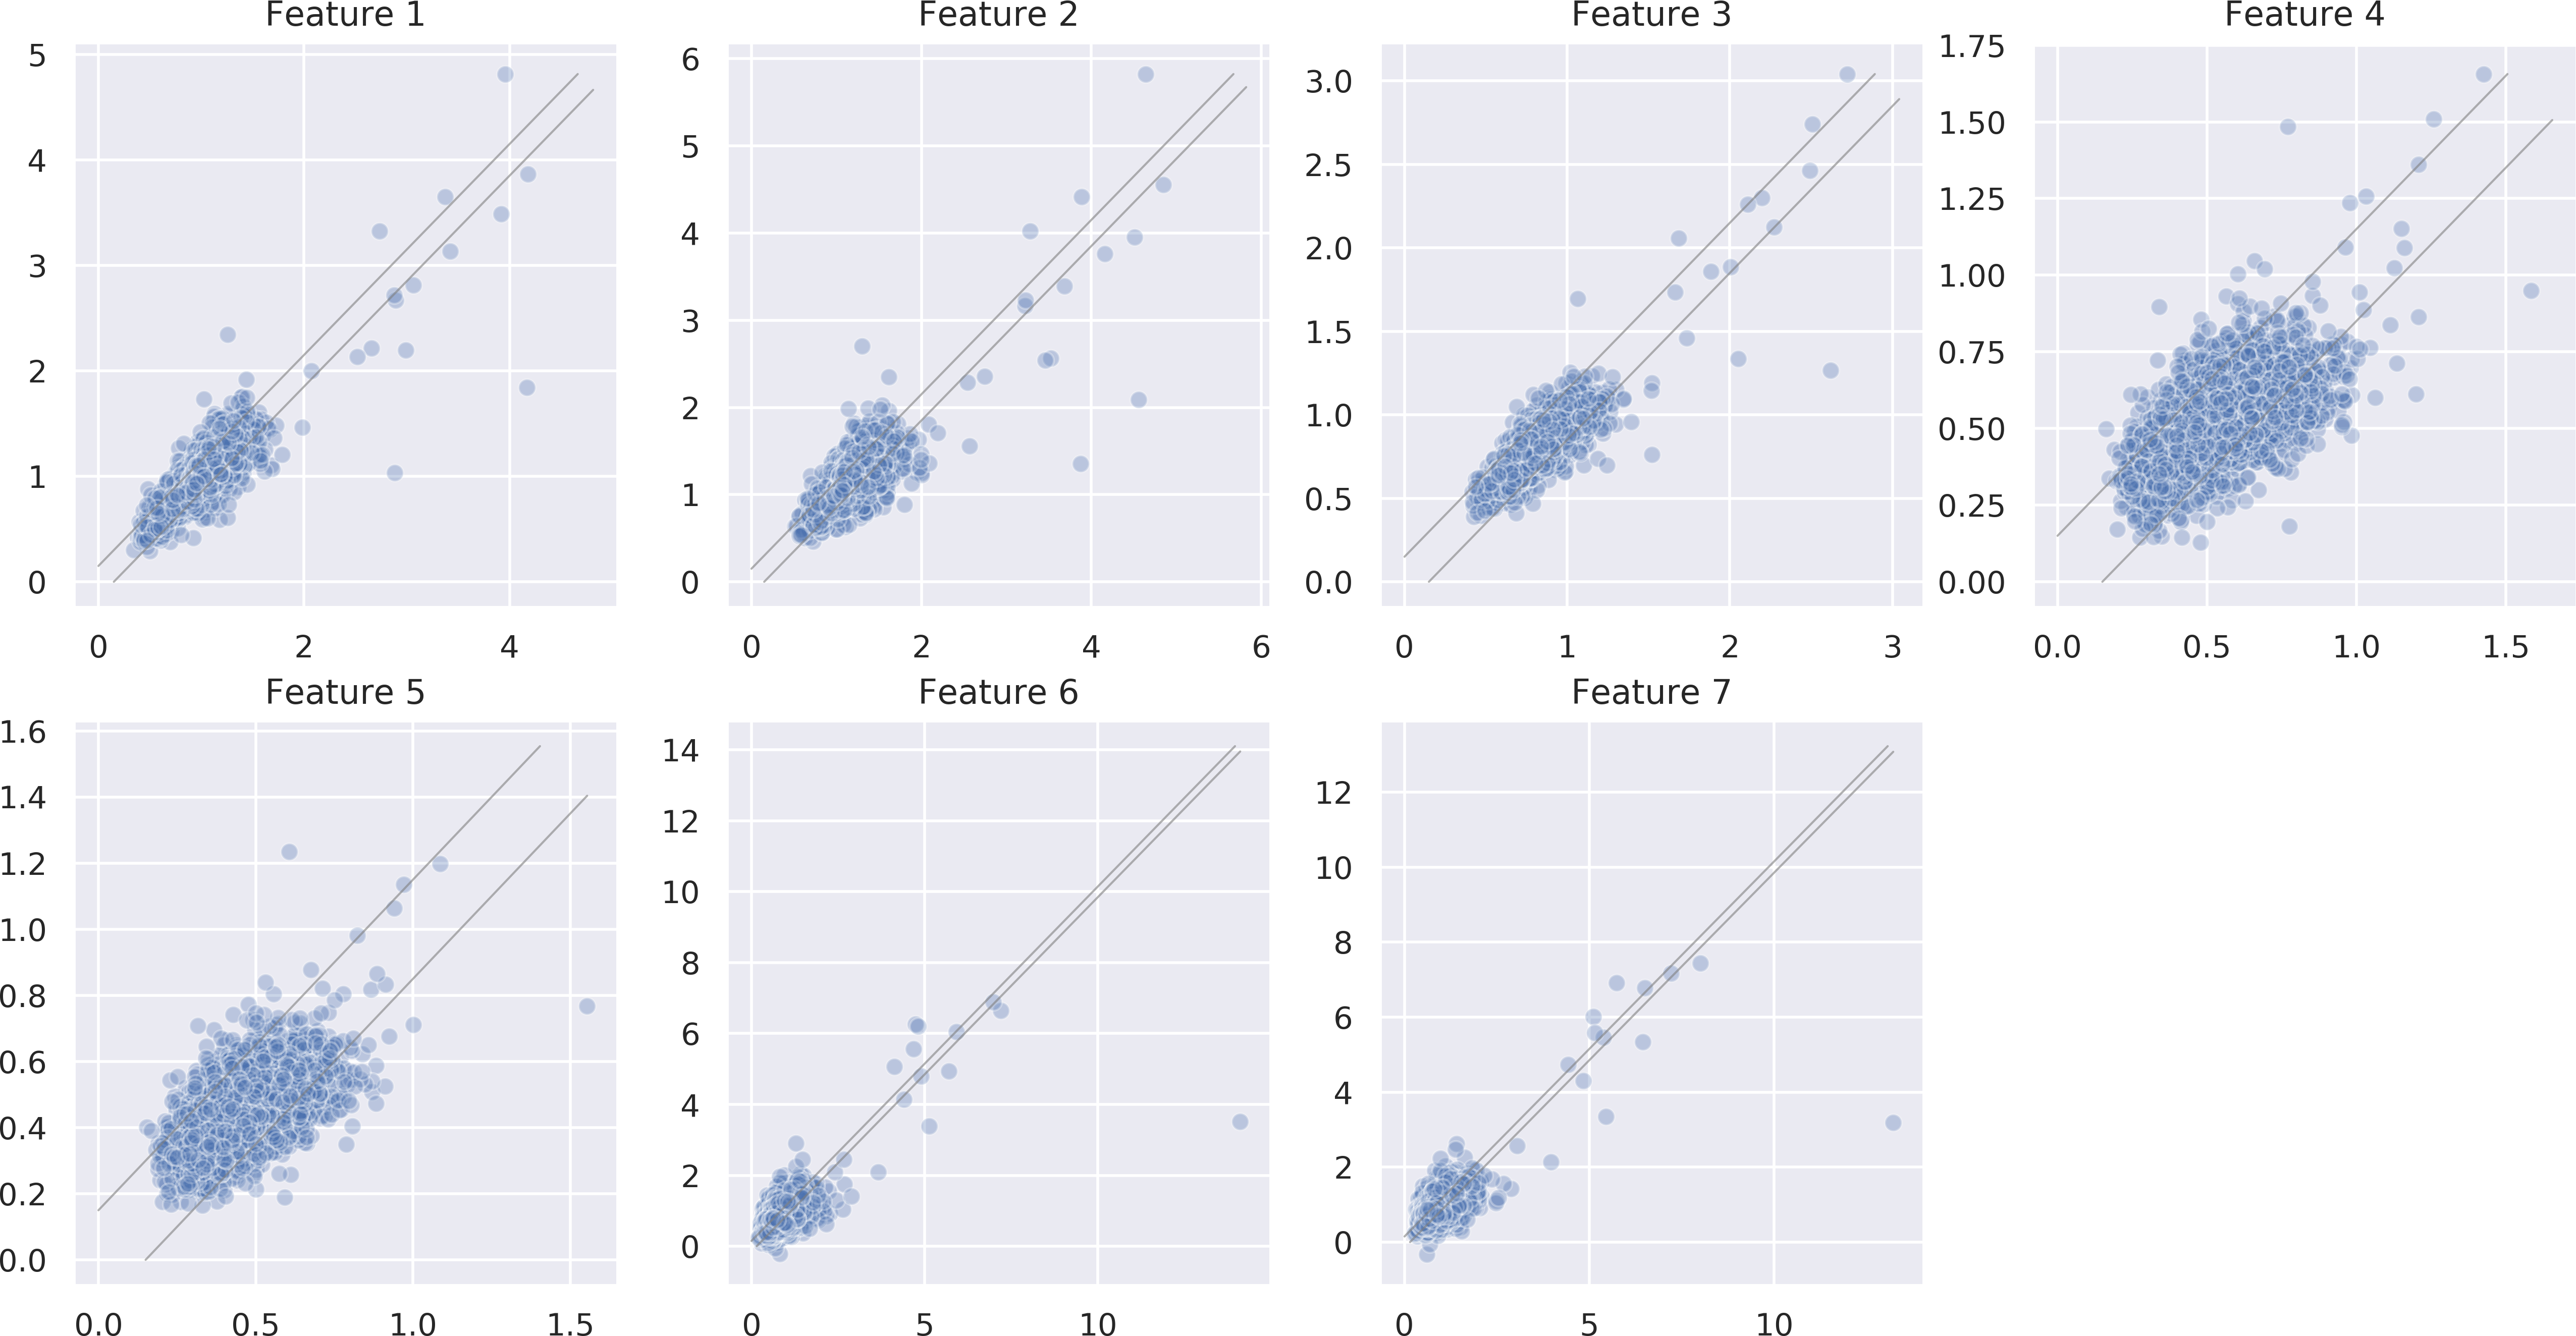
\includegraphics[width=\textwidth]{mlp_mts_reg_scatter}
    \caption{\label{fig:mlp_mts_reg_scatter} Scatter plots of \(Y_\text{true}\) (\(x\)-axis) versus \(Y_\text{pred}\) (\(y\)-axis) from the complete concatenated time series dataset for all seven features, as predicted by the \ac{mlp}. Diagonal lines represent the \(\pm0.15\) tolerance for a hit.}
\end{figure}

\section{Convolutional Neural Network}
For the \ac{cnn} model, code was adapted from the online repository\footnote{\url{https://github.com/hfawaz/InceptionTime}} created and published by \citet[]{fawaz_inceptiontime_2019}. Two types of task were attempted: time series classification and regression.

This model was trained to predict one of four classes ranging from 0 to 3 per feature. The input from each sample was an \ac{mts} with shape \(\left(4,\,81\right)\).

% TODO However, due to the equally spaced categorisation, it carries the potential benefit of amplifying the differences between the 99.5\% of flights (Section \ref{sec:cyclecounter}) that resulted in fewer than two cycles of damage, which may otherwise prove difficult to discern from one another (\ref{sec:model:mlpreg:mts}).

Results are shown in Tables \ref{tab:4cat:comp}, \ref{tab:4cat:red} and \ref{tab:4cat:vred}; the accuracy of the class predictions in comparison to the Cycle Counter values, calculated as \(\left|Y_\text{pred} - Y_\text{true}\right|\), are shown in Figure \ref{fig:classif_pred_hist}.

\begin{table}
    \begin{center}
        \caption{\label{tab:4cat:comp} Results from the \ac{cnn} classification on multivariate time series with the complete dataset (\(\text{MHR} = 0.467\)).}
        \begin{tabular}{ >{\bfseries}c c c c c c c c }
            \multirow{2}{*}{\textbf{Measure}} & \multicolumn{7}{c}{\textbf{Feature number}} \\
            & 1 & 2 & 3 & 4 & 5 & 6 & 7 \\
            \midrule
            MAE & 0.439 & 0.507 & 0.5 & 0.596 & 0.651 & 0.742 & 0.755 \\
            HR  & 0.588 & 0.541 & 0.546 & 0.452 & 0.418 & 0.363 & 0.36 \\
            \\
        \end{tabular}

        \caption{\label{tab:4cat:red} Results from the \ac{cnn} classification on multivariate time series with the reduced dataset (\(\text{MHR} = 0.437\)).}
        \begin{tabular}{ >{\bfseries}c c c c c c c c }
            \multirow{2}{*}{\textbf{Measure}} & \multicolumn{7}{c}{\textbf{Feature number}} \\
            & 1 & 2 & 3 & 4 & 5 & 6 & 7 \\
            \midrule
            MAE & 0.502 & 0.621 & 0.464 & 0.682 & 0.669 & 0.785 & 0.811 \\
            HR  & 0.554 & 0.464 & 0.581 & 0.409 & 0.405 & 0.329 & 0.316 \\
            \\
        \end{tabular}

        \caption{\label{tab:4cat:vred} Results from the \ac{cnn} classification on multivariate time series with the greatly reduced dataset (\(\text{MHR} = 0.376\)).}
        \begin{tabular}{ >{\bfseries}c c c c c c c c }
            \multirow{2}{*}{\textbf{Measure}} & \multicolumn{7}{c}{\textbf{Feature number}} \\
            & 1 & 2 & 3 & 4 & 5 & 6 & 7 \\
            \midrule
            MAE & 0.56 & 0.695 & 0.623 & 0.801 & 0.798 & 0.927 & 0.894 \\
            HR  & 0.5 & 0.407 & 0.46 & 0.325 & 0.358 & 0.278 & 0.301 \\
            \\
        \end{tabular}
    \end{center}
\end{table}

\begin{figure}
    \centering
    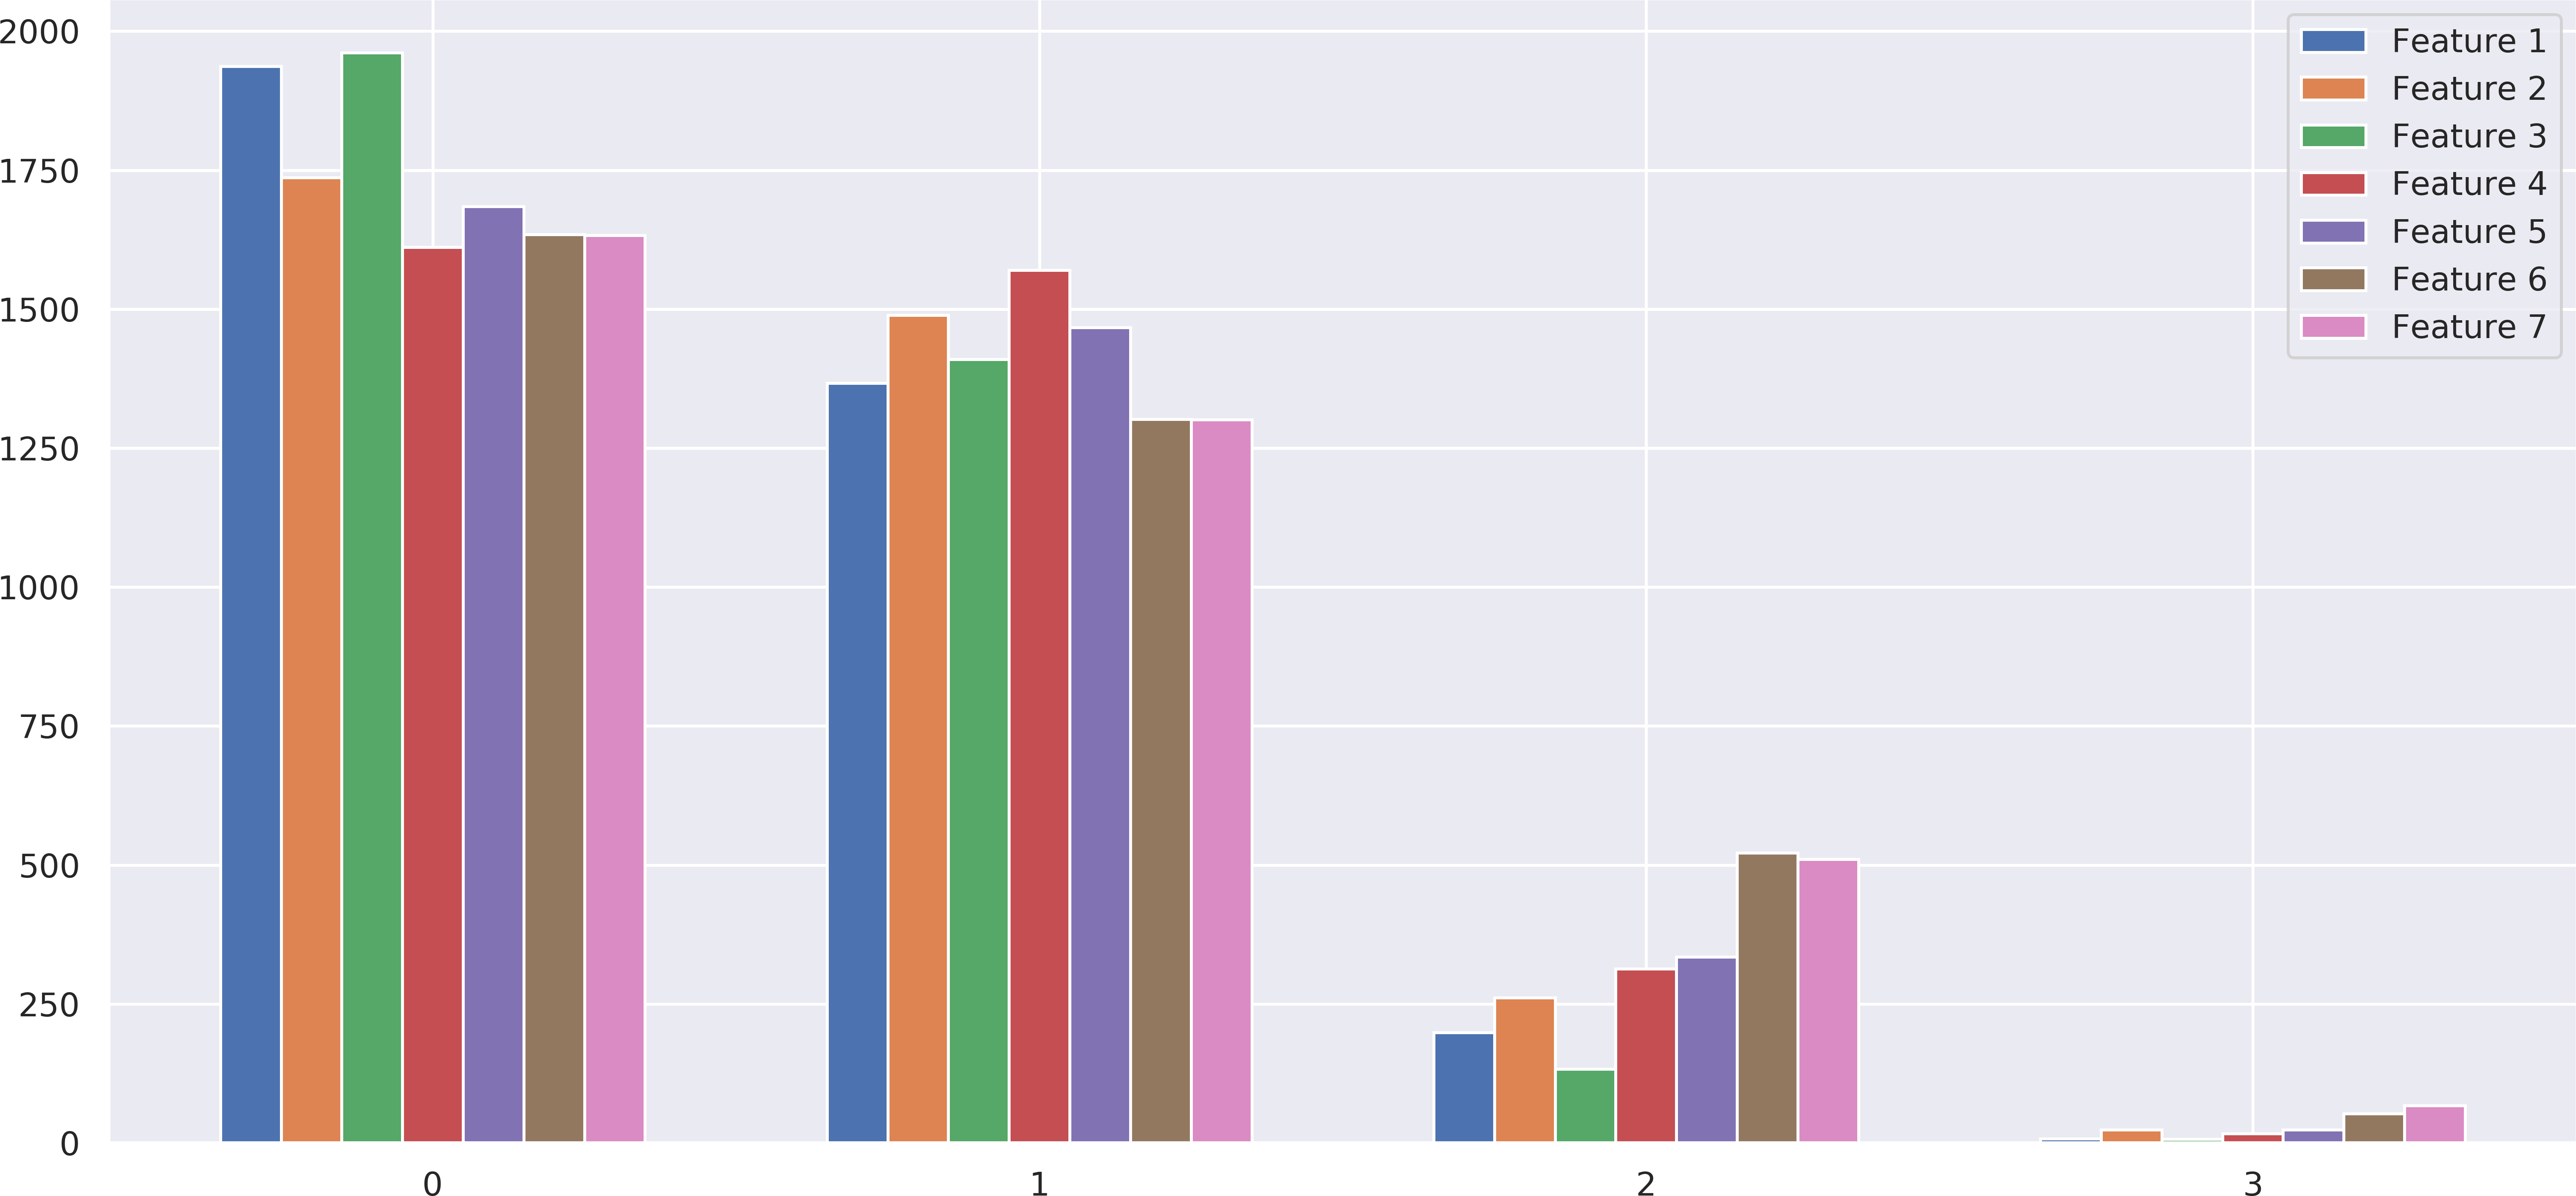
\includegraphics[width=\textwidth]{4cat_err_bar_complete}
    \caption{\label{fig:classif_pred_hist} Bar plot of absolute errors by feature from the \ac{cnn} classification model trained with the complete dataset.}
\end{figure}

\subsection{Regression: Multivariate Time Series}
By changing the activation function of the output layer from softmax to \ac{relu}, the InceptionTime classifier was converted into a regressor to be trained on the original Cycle Counter values.

Results from this model are shown in Tables \ref{tab:mts_lin:comp}, \ref{tab:mts_lin:red} and \ref{tab:mts_lin:vred}; predictions \(Y_{\text{pred}}\) are plotted against Cycle Counter values \(Y_{\text{true}}\) in Figure \ref{fig:incep_mts_reg_scatter}

\begin{table}
    \begin{center}
        \caption{\label{tab:mts_lin:comp} Results from the \ac{cnn} regression on multivariate time series with the complete dataset (\(R^2 = 0.595\), \(\text{MHR} = 0.782\)).}
        \begin{tabular}{ >{\bfseries}c c c c c c c c }
            \multirow{2}{*}{\textbf{Measure}} & \multicolumn{7}{c}{\textbf{Feature number}} \\
            & 1 & 2 & 3 & 4 & 5 & 6 & 7 \\
            \midrule
            MAE & 0.083 & 0.099 & 0.067 & 0.099 & 0.079 & 0.195 & 0.193 \\
            % MSE & 0.013 & 0.02 & 0.008 & 0.015 & 0.01 & 0.092 & 0.085 \\
            HR  & 0.892 & 0.842 & 0.952 & 0.827 & 0.911 & 0.521 & 0.527 \\
            \\
        \end{tabular}

        \caption{\label{tab:mts_lin:red} Results from the \ac{cnn} regression on multivariate time series with the reduced dataset (\(R^2 = 0.463\), \(\text{MHR} = 0.726\)).}
        \begin{tabular}{ >{\bfseries}c c c c c c c c }
            \multirow{2}{*}{\textbf{Measure}} & \multicolumn{7}{c}{\textbf{Feature number}} \\
            & 1 & 2 & 3 & 4 & 5 & 6 & 7 \\
            \midrule
            MAE & 0.103 & 0.118 & 0.071 & 0.103 & 0.081 & 0.209 & 0.211 \\
            % MSE & 0.039 & 0.066 & 0.009 & 0.017 & 0.01 & 0.086 & 0.083 \\
            HR  & 0.808 & 0.754 & 0.917 & 0.771 & 0.88 & 0.486 & 0.466 \\
            \\
        \end{tabular}

        \caption{\label{tab:mts_lin:vred} Results from the \ac{cnn} regression on multivariate time series with the greatly reduced dataset (\(R^2 = 0.677\), \(\text{MHR} = 0.843\)).}
        \begin{tabular}{ >{\bfseries}c c c c c c c c }
            \multirow{2}{*}{\textbf{Measure}} & \multicolumn{7}{c}{\textbf{Feature number}} \\
            & 1 & 2 & 3 & 4 & 5 & 6 & 7 \\
            \midrule
            MAE & 0.079 & 0.1 & 0.067 & 0.085 & 0.072 & 0.164 & 0.159 \\
            % MSE & 0.01 & 0.016 & 0.007 & 0.013 & 0.009 & 0.045 & 0.042 \\
            HR  & 0.93 & 0.868 & 0.969 & 0.9 & 0.943 & 0.641 & 0.653 \\
            \\
        \end{tabular}
    \end{center}
\end{table}

\begin{figure}
    \centering
    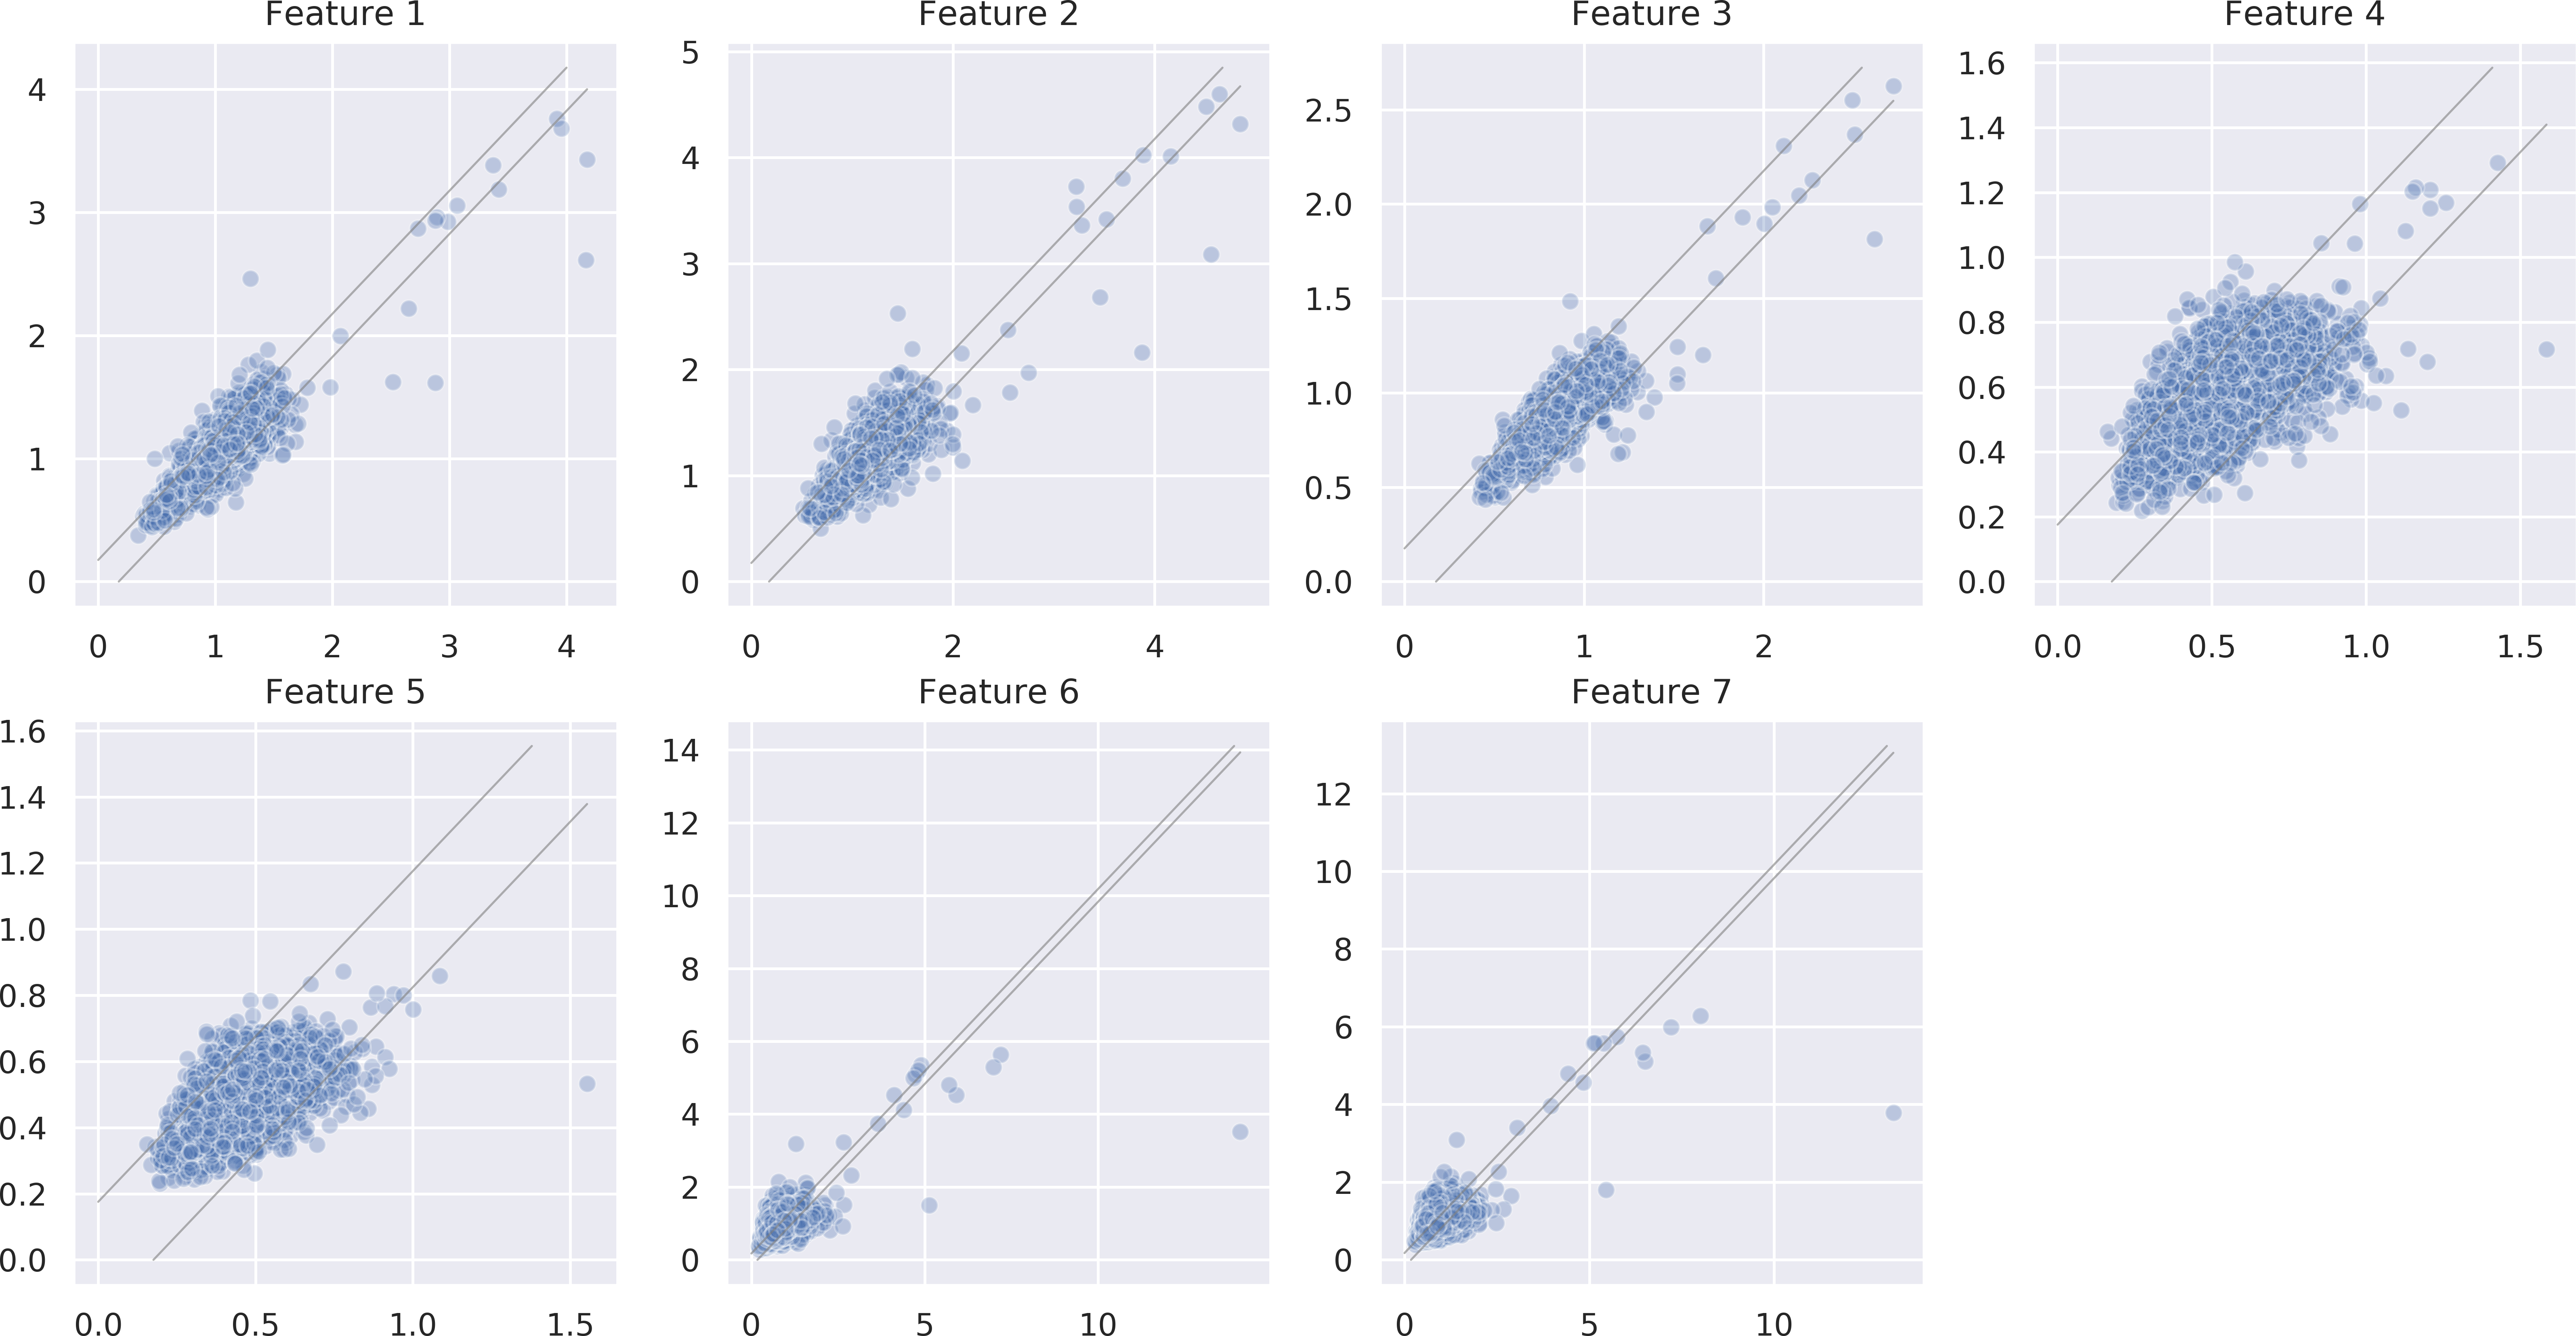
\includegraphics[width=\textwidth]{incep_mts_reg_scatter}
    \caption{\label{fig:incep_mts_reg_scatter} Scatter plots of \(Y_\text{true}\) (\(x\)-axis) versus \(Y_\text{pred}\) (\(y\)-axis) from the complete \ac{mts} dataset for all seven features, as predicted by the InceptionTime regressor. Diagonal lines represent the \(\pm0.15\) tolerance for a hit.}
\end{figure}

\section{Summary}
A summary of the main results from all models is shown in \ref{tab:model_summary}.

\begin{table}
    \renewcommand{\arraystretch}{1.25}
    \begin{center}
        \caption{\label{tab:model_summary} A summary of mean hit rates from all seven models for all dataset sizes. \(R^2\) is reported for regression models; mean absolute error is included for the classification model. The highest values of measures \(R^2\) and MHR for each dataset size are formatted in bold.}
        \begin{tabular}{ >{\bfseries}m{0.2\textwidth} m{0.15\textwidth} >{\centering}m{0.1\textwidth} >{\centering}m{0.13\textwidth} >{\centering}m{0.13\textwidth} >{\centering\arraybackslash}m{0.13\textwidth} }
            \multirow{2}{*}{\textbf{Model}} & \multirow{2}{*}{\textbf{Dataset}} & \multirow{2}{*}{\textbf{Measure}} & \multicolumn{3}{c}{\textbf{Dataset Size}} \\
            & & & complete & reduced & greatly reduced \\
            \midrule
            \multirow{4}{=}{Polynomial regression}  & \multirow{2}{=}{Key values}               & MHR       &
                0.810 & 0.789 & 0.748 \\
                                                    &                                           & \(R^2\)   &
                0.252 & 0.064 & -0.198 \\ \cline{2-6}
                                                    & \multirow{2}{=}{Key values and features}  & MHR       &
                \textbf{0.977} & \textbf{0.968} & \textbf{0.974} \\
                                                    &                                           & \(R^2\)   &
                \textbf{0.893} & 0.864 & \textbf{0.850} \\ \cline{1-6}
            \multirow{6}{=}{MLP regression}         & \multirow{2}{=}{Key values}               & MHR       &
                0.801 & 0.781 & 0.771 \\
                                                    &                                           & \(R^2\)   &
                0.474 & 0.128 & -0.272 \\ \cline{2-6}
                                                    & \multirow{2}{=}{Key values and features}  & MHR       &
                0.970 & 0.962 & 0.949 \\
                                                    &                                           & \(R^2\)   &
                0.890 & \textbf{0.865} & 0.740 \\ \cline{2-6}
                                                    & \multirow{2}{=}{Concatenated time series} & MHR       &
                0.799 & 0.790 & 0.785 \\
                                                    &                                           & \(R^2\)   &
                0.301 & 0.357 & 0.360 \\ \cline{1-6}
            \multirow{2}{=}{CNN regression}         & \multirow{2}{=}{Multivariate time series} & MHR       &
                0.782 & 0.726 & 0.843 \\
                                                    &                                           & \(R^2\)   &
                0.595 & 0.463 & 0.677 \\ \cline{1-6}
                \multirow{2}{=}{CNN classification} & \multirow{2}{=}{Multivariate time series} & MHR       &
                0.467 & 0.437 & 0.376 \\
                                                    &                                           & MAE   &
                0.599 & 0.648 & 0.757 \\
        \end{tabular}
    \end{center}
\end{table}